\chapter{Contributions}
\section{Submodules and Specifications}
%%talk about the specs


The main focus of this thesis will be on 2 important submodules in charge of their load instructions:\\

\textit{Load Buffer} and \textit{Load Management Unit}.

\subsection{Load Management Unit}
%general


This module is in charge of handling the load operations.
Those can be strided or indexed.\\

Since the VPU is able to work out-of-order an ID system is necessary, so each instructions comes with an ID.
In particular the load operation come with the signal \textbf{seq\+id\+i}.
This signal contains all the informations about the issued load.\\

The main elements of this submodules are:
\begin{itemize}
    \item \textit{Shifter}: it is useful to have the first bit not in the MSB or LSB position.
    
    \item \textit{Compactor}: it is useful to compact all the valid elements. When the stride = 1 there is no use of the compactor.
    
    \item \textit{Aligner}: it is in charge to align the elements for the output (lane, bank and sub-bank).
\end{itemize}

\bigskip

%params
The main parameters defining this submodule are:
\begin{itemize}
    \item \textbf{MEM\+DATA\+WIDTH}: width of the chunk of data received from Avispado. The standard value is \textit{512}.
    
    \item \textbf{SEQ\+ID\+WIDTH}: width of the \textit{seq\+id\+i} that identifies the data coming from Avispado. The standard value is \textit{33}.
    
    \item \textbf{MAX\+NUMBER\+ELEMENTS}: maximum number of elements that can be encoded in the chunk of data received (64 when SEW = 8 bit). The standard value is \textit{64}.
    
    \item \textbf{MAVISPADO\+LOAD\+MASK\+WIDTH}: Indicates the maximum number of mask bits that are received with the data. Every bit of the mask represent a byte into the data. The standard value is \textit{64}.
    
    \item \textbf{NUM\+LANES}: number of lanes. The standard value is \textit{8}.
\end{itemize}

\subsubsection{Interface}
%interface
%%%%%%%%%%%%%%%%TABLE%%%%%%%%%%%%%%%%%%%%%%%

\begin{table}[H]
\centering
\begin{tabular}{|l|l|}
\hline
\rowcolor[HTML]{EFEFEF} 
\multicolumn{1}{|c|}{\cellcolor[HTML]{EFEFEF}Signal} & \multicolumn{1}{c|}{\cellcolor[HTML]{EFEFEF}Description}                      \\ \hline
load\+granted\+i    & a load is granted,\\
                    & it will have a certain sew\+i and stride\+i\\ \hline
load\+granted\+sb\+id\+i    & the id for the issued Load,\\
                            & can be issued up to 2 loads\\ \hline
indexed\+load\+granted\+i   & the granted load is indexed \\ \hline
load\+data\+valid\+i        & indicates if the data in load\+data\+i bus is valid\\ \hline
load\+data\+i               & data received from Avispado\\ \hline
seq\+id\+i                  & the sequence id (described below)\\ \hline
mask\+valid\+i              & validity of mask\+i signal\\ \hline
mask\+i                     & mask bits to mask load\+data\+i\\ \hline
sew\+i                      & identifies the size of each vector element\\ \hline
stride\+i                   & stride indicated in bytes\\ \hline
load\+data\+o               & output data sent to the lanes\\ \hline
load\+dvalid\+o             & indicates if the data in load\+data\+o bus is valid\\ \hline
mask\+o                     & mask bits to mask load\+data\+o\\
                            & it is needed also for not masked inst.\\ \hline
element\+ids\+o             & identifies each element sent in load\+data\+o\\ \hline
sb\+id\+o                   & identifies the instruction\\ \hline
vstart\+self\+o             & identifies the first valid element\\
                            & in the chunk of data received in load\+data\+i\\ \hline
vstart\+next\+o             & identifies the last valid element \\
                            & in the chunk of data received in load\+data\+i\\ \hline
min\+element\+id\+idx\+o    & index of the first valid \\
                            & element in elements\+ids\+o of each lane.\\ \hline
\end{tabular}
\end{table}


\subsubsection{Sequence ID}
The sequence id ID is very useful as the memory system does not guarantee the in-order arrival of elements. So this signal contains all the info needed to correctly elaborate the data.\\

It i composed as:
\begin{itemize}
    \item \textbf{seq\+id\+i[4:0]} = \textit{v\+reg}, identifies the logical vector register that the data should be written to;
    
    \item \textbf{seq\+id\+i[15:5]} = \textit{el\+id}, identifies the lowest valid element id contained in the chunk of data being transmitted;
    
    \item \textbf{seq\+id\+i[21:16]} = \textit{el\+off}, identifies the offset in the chunk of data being transmitted.
    
    \item \textbf{seq\+id\+i[28:22]} = \textit{el\+count}, identifies the number of valid elements being transmitted. Masked elements are valid elements; 
    
    \item \textbf{seq\+id\+i[32:29]} = \textit{sb\+id}, sb\+id of the load instruction that requested the data.
\end{itemize}


\subsubsection{Handshake}
The handshake protocol with the different components is as important as the data manipulation. The following is a simple example with stride equal to 1 and offset = 0 (so, no manipulation on the data in input), also, we don't focus on how long is the vector (VLEN) so the number of elements passed from Avispado is arbitrary fixed.

\begin{enumerate}
    \item Up to 2 load are granted from the Memory Unit with the load\+granted\+i signal, and the information of sew and stride of the relative instruction are passed;
    
    \item Avispado sends the data and the seq\+id\+i with its seq\+id;
    
    \item The next clock cycle the data is on the output for the Vector Lane;
    
    \item When a load is finished, another load can be granted.
\end{enumerate}

\begin{figure}[H]
    \centering
    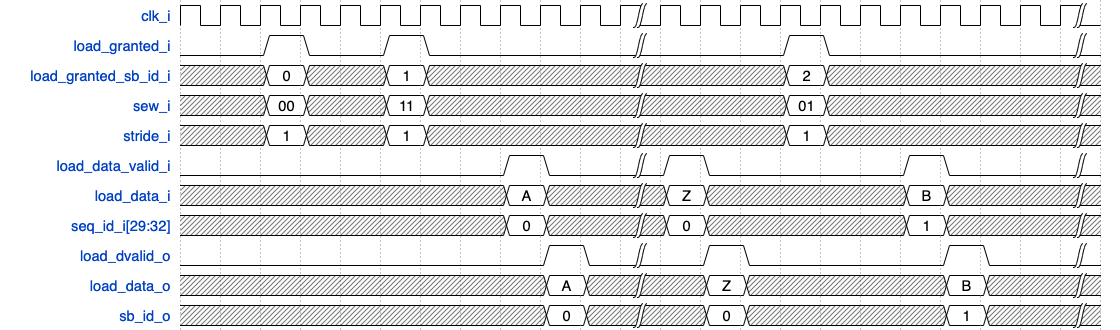
\includegraphics[scale = 0.35]{Chapter_2/img/lmu-time.png}
    \caption{Timing Diagram unit-strided load for the LMU}
    \label{lmu-time}
\end{figure}

In Figure \ref{lmu-time} it is possible to see an example for a unit-strided load. This is a simple load, and its behaviour will be discussed in the following section.

\subsubsection{Strided Load}
In this case all the valid elements are separated by a constant stride. If the stride is equal to 1, then is called unit-stride.\\

In Figure \ref{lmu-strided} there is a simple example to understand how the LMU works in this case.\\
The parameters (defined in the seq\+id\+i) are defining the elements to consider.
\begin{figure}[H]
    \centering
    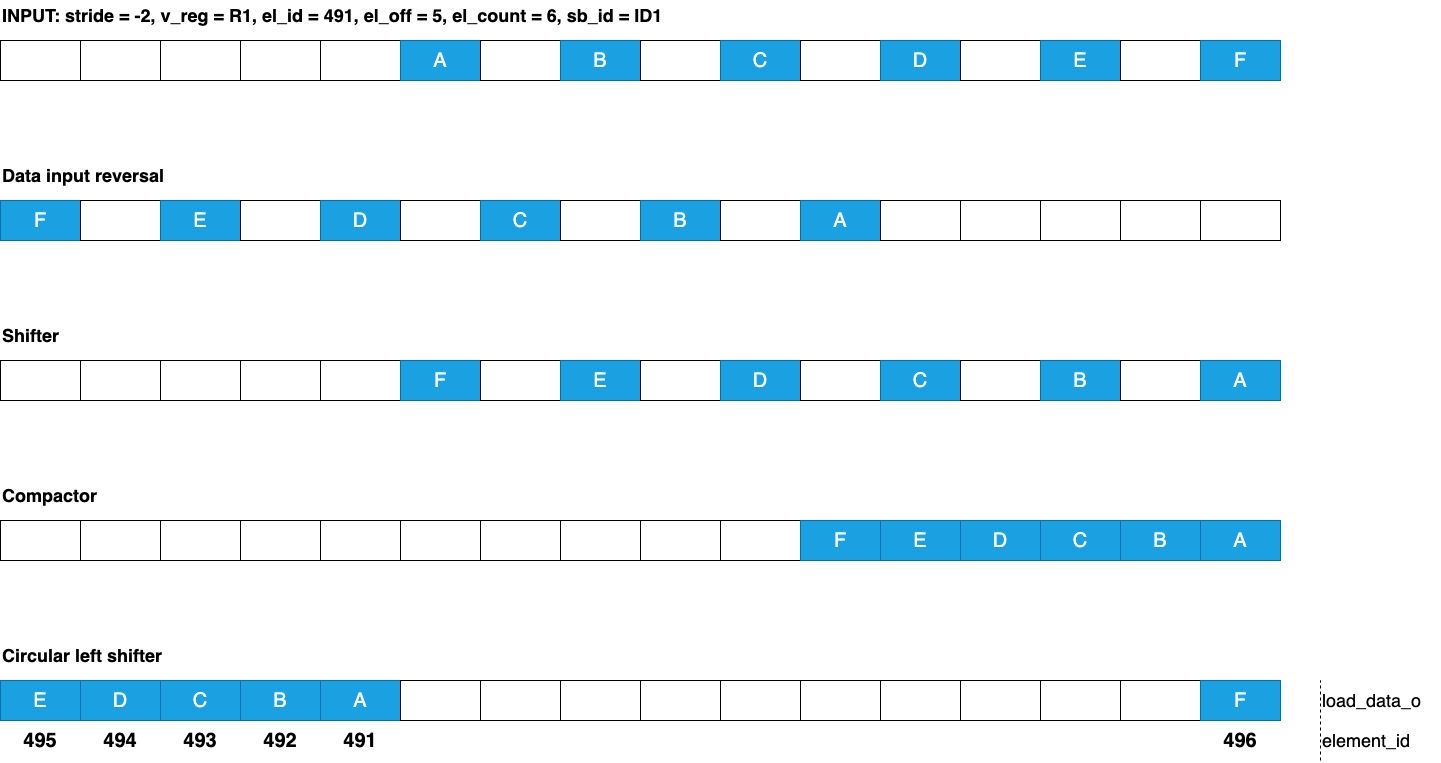
\includegraphics[scale = 0.25]{Chapter_2/img/lmu-strided.png}
    \caption{Strided load handled by the LMU}
    \label{lmu-strided}
\end{figure}

\subsubsection{Indexed Load}
It is also possible to load values in an indexed way. This means only one element at time is sent, and so the number of valid elements needs to be = 1.\\

In Figure \ref{lmu-indexed} it is possible to see an example for a simple indexed load.

\begin{figure}[H]
    \centering
    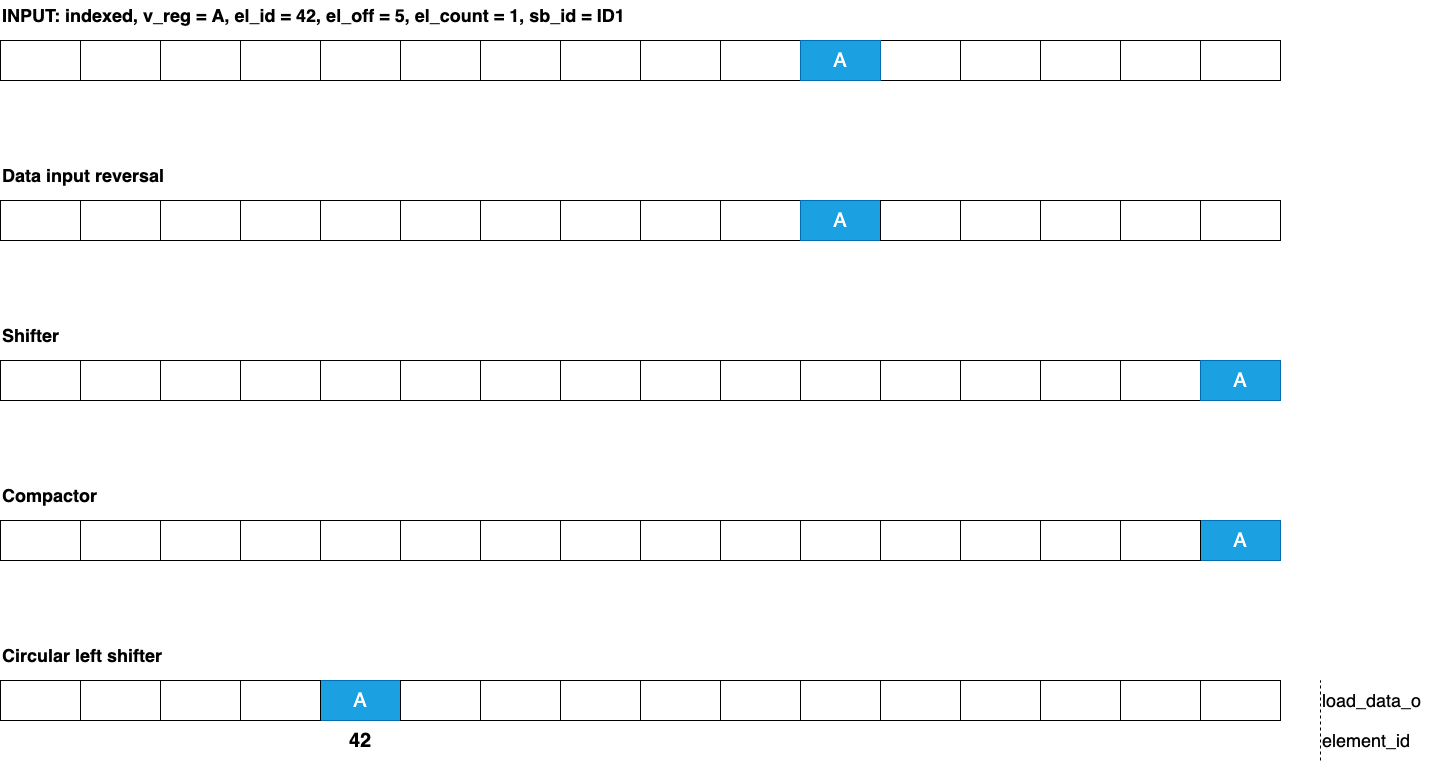
\includegraphics[scale = 0.25]{Chapter_2/img/lmu-indexed.png}
    \caption{Indexed load handled by the LMU}
    \label{lmu-indexed}
\end{figure}

\subsubsection{Masked Load}
All the load operations can be masked. This does not change the number of valid elements, but at the end of the process they not will be sent.\\


In Figure \ref{lmu-masked-stride} it is possible to see an example for the simple strided-load used before, but this time, with a mask.

\begin{figure}[H]
    \centering
    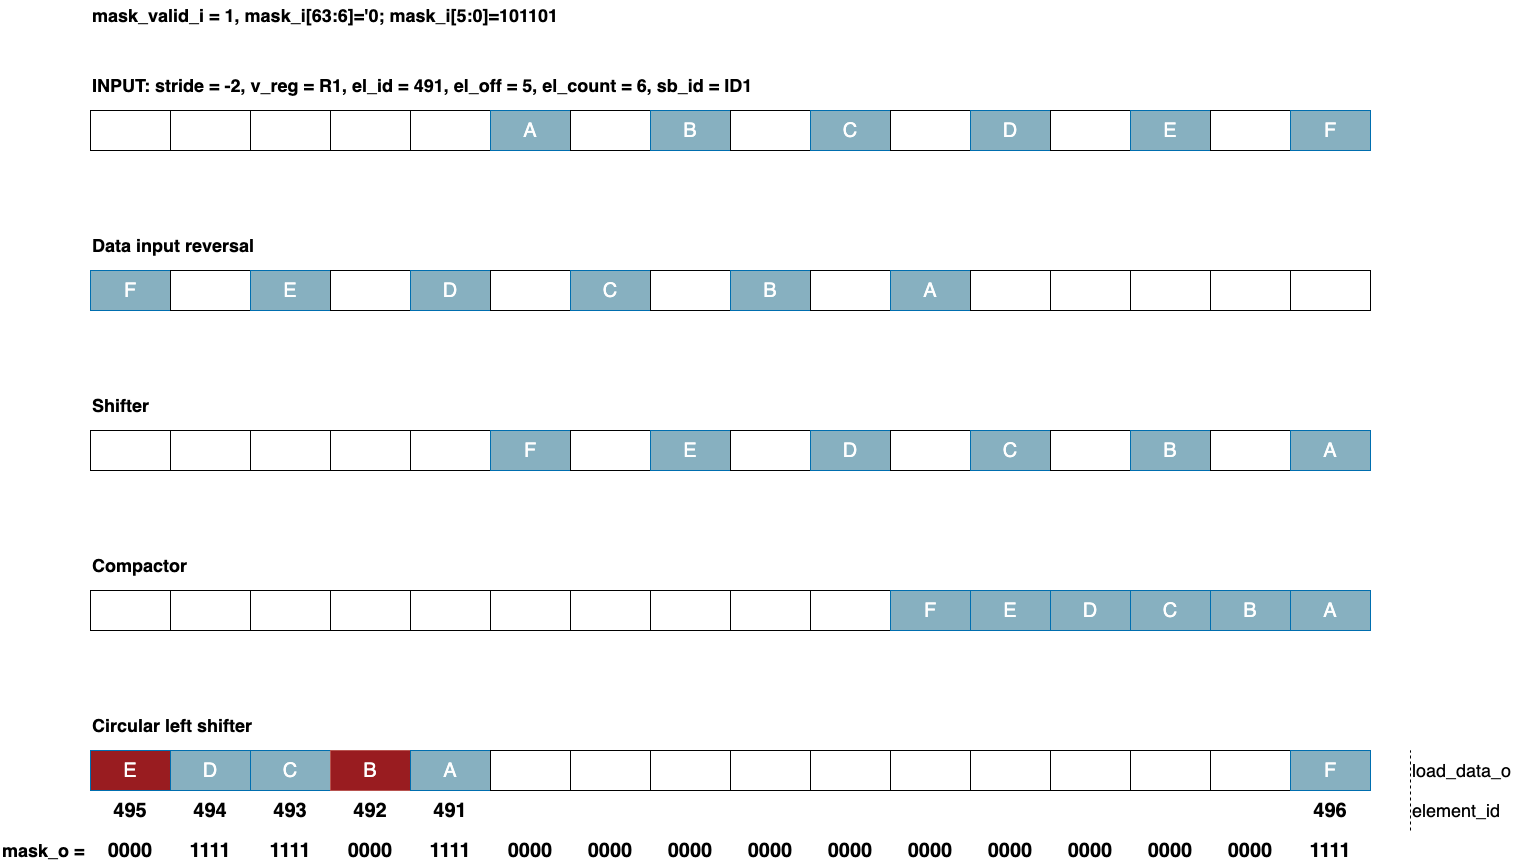
\includegraphics[scale = 0.25]{Chapter_2/img/lmu-masked-strided.png}
    \caption{Strided load, with mask, handled by the LMU}
    \label{lmu-masked-stride}
\end{figure}

\subsection{Load Buffer}
The second submodule that is mainly in charge of a load operation is the Load Buffer.\\
It is in charge of writing the data sent by Avispado to the Vector Register File. The data can be from different instructions inflight, and the Buffer will always try to optimize and group the data to write.\\

The LMU receives full cache lines of 512 bits from Avispado and forwards them to the corresponding Load Buffer for each lane (64 bits max per lane), depending on the seq\+id\+i. The position of the data into the LB will be determined by the element ID.\\

Up to 2 loads can arrive, but they can come out-of-order, although the implementation will be parameterized to accept N loads in flight.
\subsubsection{Interface}
%%tables????

\subsubsection{Structure}
There is a Load Buffer of each lane and there are 3 layers to buffer the elements. The layers are divided by the concept of Element Group. In fact the elements cannot be disposed in every combination, but every element, based on its element ID, has an exact location (based also on the sew).\\
%elements 64 e 32

In Figure there is an example for the disposition of the elements for 64 bit or 32 bit. It is also important to say the number of bit for each element group stays the same, this means the number of element depends on the sew.\\

The layers of the LB are composed mainly of 4 parts:
\begin{itemize}
    \item Elements: the elements in the buffer;
    
    \item Identifier: identifies the elements coming from the young or the old load;
    
    \item Valid: identifies if the elements are valid;
    
    \item Element Group: identifies the eg, it is assigned by considering the VRF structure.
\end{itemize}

\subsubsection{Retry}
There are cases in which 3 layers are not enough to store all the elements. Indeed it is possible that more elements have the same position and so also 4 element can cause a problem, if they try to fit.\\

This case is handled with a retry mechanism:\\
an element is discarded and a new request is made to Avispado, to  notify the retry.\\

Is important to understand the element to discard when there is a retry, if the new one or the old one.\\

There are 4 possible cases:
\begin{enumerate}
    \item if the incoming data is from the young load and the buffer only contains data from the same load, it will be discarded the data with the highest element group;
    
    \item if the incoming data is from the young load and the buffer contain data from both the oldest and youngest loads, it will discard the incoming data;
    
    \item if the incoming data is from the old load and the buffer only contains data from the same load, it will be discarded the data with the highest element group;
    
    \item if the incoming data is from the old load and the buffer contain data from both the oldest and youngest loads, it will discard the data inside the buffer, the one from the young load.
\end{enumerate}



\subsubsection{Flow}
In figure 
%schema flow
it is possible to see a simple scheme of the LB's behaviour.
%describe the flow

\section{Verification Plan}
To have a good approach with the verification of a design, it is important to define a Verification Plan.\\
There are a lot of ways to do it, and most of the times they can be automatized to better perform in long term support of them. In this specific case, the Verification Team was working along with the Design Team to produce better specifications and not only to test a completed design. This means the Verification Plan is done following the general rules to have a good value in future, but it is not entirely defined a priori.\\

It was defined before to create the UVM structure and led to the development of all the tools for the verification. \\
To define the approach to have also means to define the tools to use, in fact different of them were created:
\begin{itemize}
    \item \textbf{UVM}: is the structure described before, used to stimulate and test the DUT;
    
    \item \textbf{checkers}: are mainly composed by assertions, some really powerful statements used to define the constraints of the DUT's behaviour. \\
    They can be used in different approaches. Later on this chapter it will be discussed their use as Functional or Formal tools;
    
    \item \textbf{coverage}: is the driver of the plan. It says were to work, and were there are tests to do. 
    
\end{itemize}
\subsection{Test Plan}
To have a good coverage of the cases, and to have good reports to find bugs, it is very important to have a test plan.\\

The test plan defines all the different cases to test for a submodule or for the entire VPU. This means try to find all the different corner cases stimulating the DUT.\\

If there is the possibility a good test plan only includes different sets of stimulus, in this way an easy implementation is possible. Not in every case is in this way. For example in a submodule of the VPU not every case could be tested only modifying the inputs from the scalar core.\\
This means sometimes it is necessary to create some modified settings, to create the correct environment for the test.\\

It was created a test plan to stress the load operations. Those are affecting a lot of part of the VPU, but the focus will be on the Load Buffer, mainly.\\

\subsubsection{test on consecutive elements}
The first test planned was a simple test about consecutive elements, this means all the elements are sent in order. Of course this is a simple case, and it is thought to test if all the chain to the effective load are working. In fact it is a control test.\\

The only constraint meant to be in this test is the sequentiality of the elements.\\
An example could be the one represented in the Diagram %diagramma 0,1,2,3,4,5,6,7 con sew 64, load 0

\subsubsection{test on random values}
The second kind of test to implement is for sure the random test. This will stress the ability to use different elements ID and different loads at the same time. In this way all the handling for the positions, calculated based on the load and on the element ID, is stressed.\\

It was created a special modality to constrain the randomness to the possible values. This was implemented in the UVM using the configurations for the sequence.\\

An example could be the one represented in the Diagram %diagramma 0,3,4,10,14,7,1,13  con sew 64, load 0
%
%oppure 0, 0, 1, 1, 2, 2, 3, 3, 4, 4, 5, 5, 6, 6, 7, 7

\subsubsection{test on splitted elements} 
A very interesting case is revealed when studying the positions.\\
Let's take into account a line of elements sent by the LMU to the Load Buffer. In this case the sew needs to be different from 64, so the case will use sew = 32.\\

The data sent will be sequential starting from 65 to 80. In this way it is possible to test if the output is disposed correctly and so if the Load Buffer for the Lane[0] store 80-65 as values.\\

An example could be the one represented in the Diagram %diagramma 

\subsubsection{test on retries}
The last test typology is about the retry mechanism. This occurs when all the tree lines are fulled with an element in the same position, and thena fourth elements arrives, this means the Load Buffer doesn't have another position for the element, thus one of the elements needs to go back to the sender and a new request is made.\\

Considering sew = 64, there are different versions about this test: it can be a simple in order retry with elements 0-40-80-120-... as inputs, it can be out of order as 0-40-120-80-..., or it can be with two different loads.\\

The easy example is represented in the Diagram %diagramma 

\section{Functional Verification}
The test executed are just the base for a verification. It can be defined Functional Verification the process to verify a design agaist its specifications.\\

The approach is normally to define some functionalities and then compare them to the design. This of course is the crucial part, because it is not always obvious how a specific case works. Also there are different ways to test those functionalities.\\

\subsection{Scoreboard}
As saw into the test plan, an easy way to test the results is the scoreboard, thus to have a predicted value and then to compare it against the calculated one.\\

Before the work of this thesis a scoreboard for the entire UVM was already implemented. Let's now analyze a little bit how it works and why it was useful to develop other tests.

\subsubsection{Spike}
Spike is a RISC-V ISA Simulator and it implements a functional model of one or more RISC-V harts. For this specific project it was extended to support the vector extension.\\
It is used first to simulate the Avispado core, then the result is feed to the VPU and to the Spike vector extension. Finally the results are compared. A simple scheme is represented in Figure %scheme spike.so
\\

This kind of tool is very useful when running tests because it is faster than a specific test for each component the test is stressing, and at the same time can give hints about the working condition. Of course it is just a first step, because it will be hard to find a bug using only the comparison with the final result.\\

\subsubsection{Load Management Unit's scoreboard}
The aim of this thesis was principally based on testing the Load operations, so a scoreboard for the LMU was created.\\

Recalling the LMU working model, it first takes into account the stride, reversing the data in case of negative stride, then the data is positioned correctly again, then it is compacted considering the stride, and finally it is aligned to match with correct ID.\\

In high level it was done using vectors, and a couple of steps were merged together. It is possible to see below the pseudo code represntig the implementation in this way.

\begin{lstlisting}[language=Verilog,style=verilog-style]
        x=new[N_ELEMENTS][SEW];
        y=new[N_ELEMENTS][SEW];

        //first assignement
        x[N_ELEMETS][SEW] = load_data_i[N_ELEEMTS*SEW]

        //consider the stride
        if(stride<0 && !is_indexed)
            y[i] = x[-i];
        else
            y[i] = x[i];
        

        //from # of bytes to # of elements
        local_stride = mod(local_stride * 8 / SEW);

        //concatenate the data according to stride 
        x[N_ELEMENTS-1-i] = y[(N_ELEMENTS-1-i*local_stride-OFFSET)%N_ELEMENTS];

        //shift the data according to EL_ID
        k = EL_ID % N_ELEMENTS;
        
        y[(N_ELEMENTS-1-(k+i))%N_ELEMENTS] = x[(N_ELEMENTS-1-i)]
\end{lstlisting}

Also the mask was predicted in a similar way, thus this step was then implemented with a simple check on the mask to have the correct result.\\

In this way it is possible to have an exact result for the LMU, so when a big test fails, it is always possible to check if the LMU performed correctly with the data it received in input.\\

\subsubsection{Load Buffer's scoreboard}
For the Load Buffer the behaviour was really complicated, so a simplified  version of a scoreboard was implemented.\\

Hence it does not work on the correct result operation per operation, this because the LB has 3 layer of deepness and always tries to optimize the output. So to implement all the rules about the output would be to create a similar structure with an high risk to create a bug in the Verification model.\\

The concept was see the data in input and then expect, eventually, the same data in the correct position as output. This of course is conflicting with the concept of retry, in fact when a retry is executed it is not guaranteed the data as output.\\

It was implemented as an assertion (whose behavior will be explained in the following section), to create a time correlation.\\

A pseudo version of this checker is represented below.
\bigskip

\begin{lstlisting}[language=Verilog,style=verilog-style]
// Pseudo checker
if( lmu_dvalid_load_i) { 

    load_data_o[get_el_bank(el_id_i, sew_i)*SEW + SEW-1 -: SEW] == data_i;
}


// This function computes the bank of an element
function [BANK_IDX_SZ-1:0] get_el_bank([EL_ID_WIDTH-1:0] el_id, [SEW_WIDTH-1:0] sew);
    case (sew[1:0])
        SEW64: get_el_bank=((el_id/N_LANES)%N_BANKS); 
        SEW32: get_el_bank=(((el_id>>1)/N_LANES)%N_BANKS); 
        SEW16: get_el_bank=(((el_id>>2)/N_LANES)%N_BANKS); 
        SEW8:  get_el_bank=(((el_id>>3)/N_LANES)%N_BANKS); 
    endcase
endfunction

\end{lstlisting}
\bigskip

Using the element\+id and the corresponding bank (based on the sew), it is possible to predict the result for a specific location and compare it. In this pseudo code it is not very visible the time handling, but the if statement can wait until the result goes as output.


\subsection{Assertions}
The other powerful tool are the Assertions.\\

An assertion is a simple check on a defined functionality. It is wanted to receive an error when an assertion fails.\\
It is mainly composed by two parts both of them conditions, but they act differently and are time related. The first part is a condition to \textit{"fire"} it, this means when the condition is true the assertions starts checking for the second part.\cite{verification-book-2016}\\

The second part is another check on some condition, and can reveal the result of the check. At this point the possible results are \textit{True} or \textit{False}.\\

Both of them can be time consuming, and conditions on the edge are possible.\\
It is also possible to embed \textit{properties} and \textit{sequences} into them, in this way  a combination of all the functionality is achievable.\\

Let's now see the default structure of an assertion.

\begin{lstlisting}[language=Verilog,style=verilog-style]


property property_1;
    @(posedge clk_i)
	a |-> b;
endproperty : property_1

assertion_1 : assert property ( disable_iff(rst) property_1) else $error("")

\end{lstlisting}
\bigskip

Basically if a is HIGH(1) then it is expected that b is also HIGH(1).\\

The functionality is expressed into the property, then it is asserted into the assertion. It could be possible to recall tasks or processes, in this way a certain computation is possible.
It can also provide an error message.\\
When the reset is asserted then the assertion is disabled. This means the assertion need now to be re-fired with a new condition.\\

\subsubsection{Load Management Unit's assertions}
The main focus was on the calculated result and on the handshake with the other components.\\

In the verification plan were previously defined all the functionality to check, then a list of assertions was used to produce a good checker.\\

%%controlla appendice
The list of all the checkers can be found in Appendix B.\\

\begin{table}[H]
    \centering
    \begin{tabular}{|l|l|}
    \hline
    
    \hline
    
   \textbf{name} & \textbf{functionality} \\ \hline
   
   \hline
   
\toran a\+el\+count & when load\+data\+valid\+i \\ \toran  & then $seq\_id[28:22] (el\_count) \leq \frac{( n\_elements - el\_offset )}{(stride*8/sew)}$ \\ \hline

\tloran a\+stride \+i & $stride\cdot8$ can be one of the following $\pm{} (sew, 2\cdot sew,  4\cdot sew)$ \\\tloran & with SEW = $2^{(3+sew)}$ and not indexed load \\ \hline

\toran a\+load\+granted\+i\+known & when load\+granted\+i, \\ \toran & not unknown the following : sew, granted\+sb\+id \\ \hline

\tloran a\+load\+data\+i\+known & when data\+valid\+i, \\\tloran & not unknown seq\+id\+i, load\+data\+i \\ \hline

\toran a\+sb\+id\+o & when load\+data\+valid\+i ,\\\toran & next clock cycle sb\+id\+o(t) = seq\+id\+i[29:32](t-1) \\ \hline

\tloran a\+load\+dvalid\+o\+known \tloran & when load\+dvalid\+o, outputs known \\ \hline

\toran a\+dvalid\+o & after load\+data\+valid\+i,\\\toran & next clock cycle, load\+dvalid\+o \\ \hline

\tloran a\+vstart\+o & correct v\+start\+next\+o v\+start\+self\+o, \\\tloran &  according to load\+data\+o \\ \hline

\toran a\+granted\+ids & can't be granted 2 loads with the same id at once \\ \hline

\tloran a\+indexed\+instr & when the load is an indexed load, \\\tloran & el\+count=1 and mask\+valid\+i = 0 \\ \hline

\toran a\+load\+sync\+end\+i & for every load\+granted\+i \\\toran & there is eventually the corresponding load\+sync\+end\+i  \\ \hline

\tloran a\+load\+grant\+beh & when num\+load\+inflight = 2, load\+grant\+i = 0 \\ \hline

\toran a\+load\+sync\+end\+beh & when num\+load\+inflight = 0, load\+sync\+end\+i = 0 \\ \hline

\tloran a\+load\+req\+sync\+end & load\+sync\+end\+i cannot be simultanous with a load\+granted\+i \\ \hline

\toran a\+el\+count\+sew\+i & when $stride\_i \neq (1, 2, 4)\cdot sew\_i$ (in bytes), \\\toran & el\+count has to be = 1 \\ \hline

\hline

\tlazzu a\+sb\+correct & when load\+dvalid\+i, \\\tlazzu & if it is given a sb\+id not present in the fifo,\\\tlazzu &  load\+dvalid\+o will be 0 \\\hline

\tazzu data\+o & correct load\+data\+o, \\\tazzu & clk cycle after load\+dvalid\+i (stride/mask/indx)\\\hline

\tlazzu mask\+o & correct mask\+o, according to load\+data\+o\\\hline

\tazzu el\+ids\+o & correct element\+ids\+o\\\hline

\tlazzu a\+min\+el\+id\+idx\+o & correct min\+el\+id\+idx\+o\\\hline

\hline

\tyell a\+rsn\+o & when rsn\+i load\+dvalid\+o = 0 and mask\+o = '0 \\\hline
\tlyell a\+rsn\+i & when rsn\+i load\+data\+valid\+i = 0 \\ \tlyell & and load\+granted\+i = 0 \\\hline

    \end{tabular}
    \caption{Assertions on LMU}
    \label{tab_lmu_check}
\end{table}

As it is possible to see in Table \ref{tab_lmu_check} there are different assertions possible for a single submodule. Here they are separated by colour distinguishing the different "category". Indeed the orange ones are checking the basic signals behaviour and also the handshakes.\\
The light blue ones are scoreboard-like assertions, indeed are checking the scoreboard\+id, the data in output and also the masks.\\
The yellow ones are just checking the conditions for the reset and the expected output.\\



\subsubsection{Load Buffer's assertions}
\section{Formal Verification}

